\textbf{Цель работы:}\\1) измерение температурной зависимости  
коэффициента поверхностного натяжения дистиллированной воды с использованием 
известного коэффициента поверхностного натяжения спирта;  
\\2) определение полной поверхностной энергии  и теплоты, необходимой 
для изотермического образования единицы  поверхности жидкости  при различной 
температуре. \\\indent

\textbf{Оборудование:} прибор  Ребиндера  с термостатом и 
микроманометром; исследуемые жидкости; стаканы.

\section*{Теоретические сведения и экспериментальная установка}
\normalsize{Для сферического пузырька с воздухом  внутри жидкости 
избыточное давление даётся формулой Лапласа:}
\begin{equation}
    \Delta P = P_{\text{внутри}} - P_{\text{снаружи}} = \frac{2\sigma}{r}
\end{equation}
\normalsize{Соответсвенно эта формула и будет испльзована для определения
коэффициента поверхностного натяжения жидкости.}

\begin{figure}[b]
    \centering
    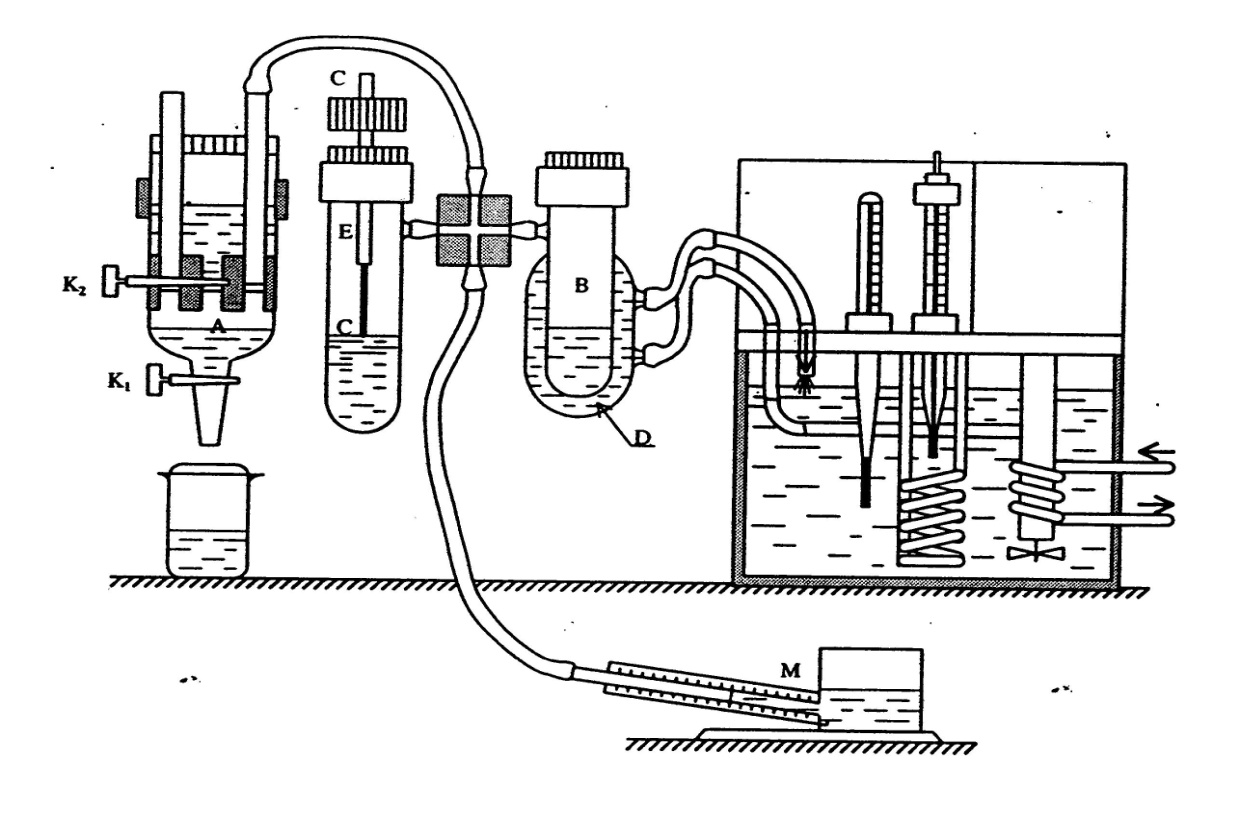
\includegraphics[height=5cm, width=10cm]{установка.jpg}
    \caption{Экспериментальная установка}
    \label{fig:experiment}
\end{figure}
\textbf{Экспериментальная установка} изображена ниже. 

В колбе E находится спирт, в колбе B - дистиллированная вода. Разряжение
в системе создается с помощью аспиратора A (вода вытикает при открытии
крана K1). А разность давлений измеряется спиртовым микроманометром М\\ \indent
Поверхностное натяжение можно определить по величине разряжения
$\Delta P$, необходимого для прохождения пузырьков при известном радиусе
иглы.\\ \indent
Стабилизация температуры воды происходит через рубашку D колбы, в
которой непрерывно прогоняется вода из термостата.\\ \indent
Чтобы устранить погрешность в измерении давления при погружении 
иглы ( 1) температура на конце металлической трубки заметно ниже, чем
в глубине жидкости; 2) тепловое расширение поднимает уровень жидкости)
погрузим кончик трубы на самое дно. Тогда давление, измеренное
микрометром, будет $P = \Delta P + \rho g h$. Последнее слагаемое
измерим двумя способами:\\
1) замерим величину $P_1$, когда кончик трубы только касается поверхности
жидкости. После опустить иглу до дна и замерить $P_2$. Разность
$P_2 - P_1$ и есть $\rho g h$;\\ 
2) измерить линейкой глубину погружение иглы  $h$. 
\section*{Экспериментальные данные}
Игла опущена до прикосновения со спиртом. Таблица максимальных давлений
при пробулькивании изображена ниже.
\begin{table}[h]
    \centering
    \begin{tabular}{|c|c|c|c|}
        \hline
        № & 1 & 2 & 3 \\ \hline
        $\Delta P_{\text{спирт}}$, Па & 78.48 & 76.518 & 78.48 \\ \hline
    \end{tabular}
    \caption{Максимальное давление при пробулькивании пузырьков
            воздуха через спирт}
\end{table}

$$\sigma_{\text{P}} = \sqrt{\frac{\sum_{i=1}^{N} (P_{\text{ср}}-P_{\text{i}})^2}{N-1}+{\sigma_{\text{инстр}}}^2}$$
$$\sigma_{\text{инстр}} = 0.2 \text{ Па}$$
$$\Delta P_{\text{спирт}} = 77.80 \pm 0.95 \text{ Па}$$

Определим диаметр иглы:\\
\textbf{1)С помощью микроскопа:}
$d_{\text{игл}} = 1.05 \pm 0.05\text{ мм} (\approx 5\%)$\\
\textbf{2)По формуле :}
$d_{\text{иглы}} = 1.17  \pm  0.1\text{ мм}  (\approx 5.8 \%)$, где 
$\sigma_\text{d} = \frac{\sigma_\text{P}}{\rho g} = 0.1 \text{ мм}$\\

Опустим иглу в проибирку с водой до касания поверхности жидкости и измерим 
максимальное давление $P_1$, при котором происходит пробулькивание.
Теперь утопим иглу до предела и так же измерим давление $P_2$.
\begin{table}[h]
    \centering
    \begin{tabular}{|c|c|c|c|c|c|c|}
        \hline
        \text{Величины} & $P_1, \text{Па}$ & $P_2\text{, Па}$ & $h_1\text{, мм}$ & $h_2\text{, мм}$ & $h_1 - h_2\text{, мм}$ & $\frac{P_2-P_1}{\rho g}\text{, мм}$ \\ \hline
        \text{Данные} & 209.2 & 315.84 & 18 $\pm 1$ & 7 $\pm 1$ & 11 $\pm 2$ & 10.9 $\pm 0.14$ \\ \hline
    \end{tabular}
    \caption{Максимальное давление при пробулькивании воду при различных
    положениях иглы}
\end{table}
$$\sigma_{\Delta h} = \frac{\sqrt{2}\sigma_{P}}{\rho g} = 0.14 \text{ мм}$$

Теперь снимем зависимость $\sigma (T)$ дистиллированной воды.
Время установления заданной тепмературы в колбе с водой большое, поэтому
после достижения указанной на термостате температуры необходимо еще в течение
5-7 минут подождать достижения равновесия в жидкости.
\begin{table}[h]
    \centering
    \begin{tabular}{|c|c|c|c|c|c|c|c|c|}
        \hline
        $P$& 163 & 166 & 167 & 171 & 169 & 167 & 166 & 165 \\
         & 164 & 166 & 167 & 170 & 169 & 167 & 166 & 165 \\
         & 164 & 166 & 166 & 171 & 170 & 166 & 166 & 165\\ \hline
        $T^\circ C$ & 25 & 30 & 35 & 40 & 45 & 50 & 55 & 60 \\ \hline
    \end{tabular}
    \caption{Зависимость давления воды от температуры}
\end{table}


\begin{figure}[h]
    \centering 
    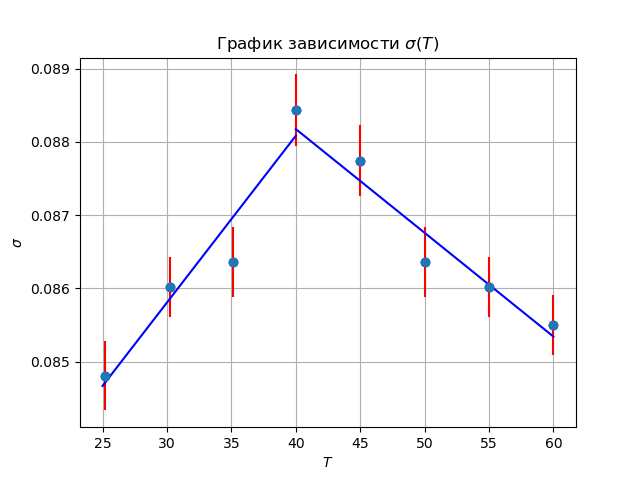
\includegraphics[height=10cm]{plot1.png} 
    \caption{График зависимости $\sigma (T)$ поверхностного натяжения 
            воды от температуры} 
    \label{fig:sigmaT} 
\end{figure} 
$k1 = 22*10^{-5}$ Н/(м$^\circ C$);     
$k2 = 14*10^{-5}$ Н/(м$^\circ C$)\\

\begin{figure}[h!]
    \centering 
    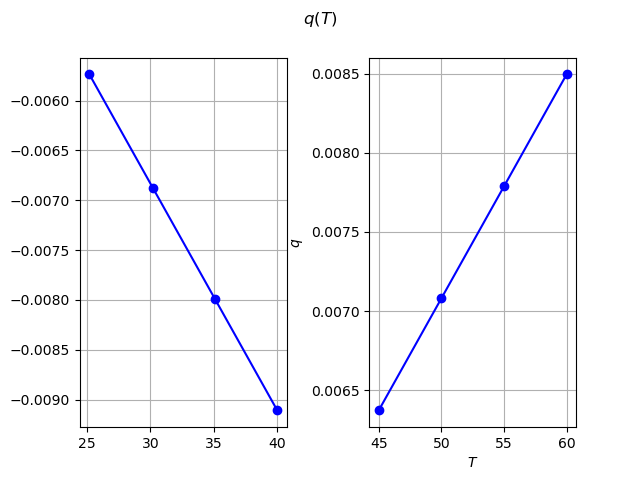
\includegraphics[height=10cm]{plot2.png} 
    \caption{График зависимости $q (T)$ теплоты образования единицы  
            поверхности жидкости от температуры} 
    \label{fig:qT} 
\end{figure} 

\begin{figure}[h!]
    \centering 
    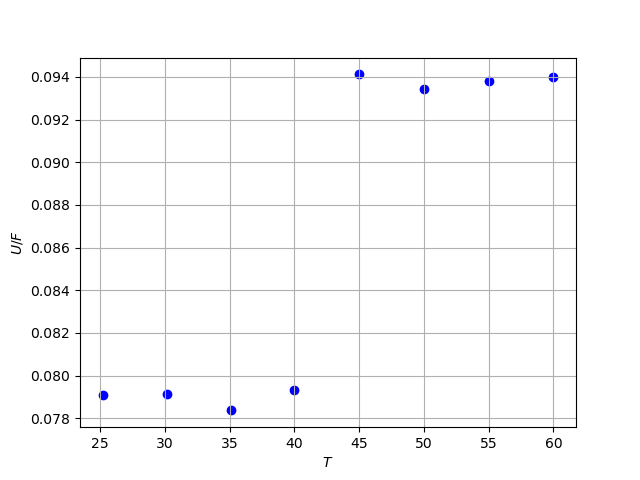
\includegraphics[height=10cm]{plot3.png} 
    \caption{График зависимости $\frac{U}{F} (T)$ поверхностной 
            энергии единицы воды от температуры} 
    \label{fig:uT} 
\end{figure} 

\section*{Выводы и результаты}
\textbf{1)Сравнение диаметров иглы, полученных с помощью микроскопа и измерений:}\\
Диаметр иглы, посчитанный по формуле получился порядка 1мм, что в пределах погрешности
совпадает с измерениями на микроскопе. \\
\textbf{2)Cравнение разсности высот погружения иглы:}\\ 
Разность, посчитанная по формуле так же совпадает с разностью, измеренной линейкой 
в пределах погрешности. \\
\textbf{3)Зависимость коэф. повехностного натяжения воды от температуры:}\\ 
При увеличении температуры жидкости $\sigma$ должна убывать, однако в эксперименте она
сначала увеличивалась, а потом уже уменьшалась. С чем это может быть связано? 
Во-первых, из-за недостаточного времени ожидания при прогреве жидкости. Термостат показывает
текущую температуру на дне сосуда, в то время, как игла воткнута насередину возможного
погружения. Из-за чего жидкость не успевала прогреваться. Поэтому полученные данные 
нельзя считать корректными. К тому времени, как жидкость действительно начала 
прогреваться, $\sigma$ начала падачть, что можно увидеть на графике. 


